\section{Úvod do matematické optimalisace}

\subsection{Důkaz souvislosti minima a maxima}
Tvrzení. Pro $f: D \rightarrow \R, M \subseteq D, \hat{x} \in M$ platí:

\begin{enumerate}[(1)]
    \item $\hat{x} \in \underset{x \in M}{\argmin} f(x) \iff \hat{x} \in \underset{x \in M}{\argmax} (-f(x))$,
    \item jesliže $\hat{x} \in \underset{x \in M}{\argmin} f(x)$, pak $\underset{x \in M}{\min} f(x) =
    - \underset{x \in M}{\max} (-f(x))$.
\end{enumerate}
Důkaz.
\begin{enumerate}[(1)]
    \item $\hat{x} \in \underset{x \in M}{\argmin} f(x)$, tj. $f(\hat{x}) \leq f(x), 
    \forall x \in M \underset{\cdot (-1)}{\iff}
    -f(\hat{x}) \geq -f(x), \forall x \in M$,\\tj. $\hat{x} \in \underset{x \in M}{\argmax} (-f(x)). \qed$

    \item Ať $\hat{x} \in \underset{x \in M}{\argmin} f(x)$, pak $\underset{x \in M}{\min} f(x) = f(\hat{x}) =
    - (- f(\hat{x})) \overset{(1)}{=} - \underset{x \in M}{\max} (-f(x)). \qed$
\end{enumerate}

\subsection{Hledání přípustných množin}
\optAs{min}{x^2 + 1}{
    \frac{3}{x} &\leq 1, \\
    x &\in \N.}
Upravíme podmínky a uděláme jejich průnik: $(x - 3 \geq 0) \land (x \in \N) \Rightarrow M = \N \setminus \bc{1,2}$.

Úvahou pak lze uhodnout minimum - minimum leží v bodě $x=3$.

\subsection{Hledání přípustných množin}
\optAs{max}{\ln x}{%
    \cos(\pi x) &= 1,\\
    x &\leq 5.
}
$D(f) = (0, \infty)$.

Udělejme průnik definičního oboru funkce a podmínek: $(x \in (0, \infty)) \land (x \leq 5) \land (\cos(\pi x)=1)$.

\begin{multicols}{2}
  \begin{figure}[H]
    \center
    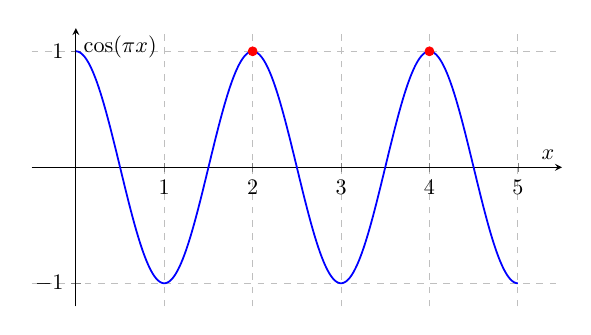
\begin{tikzpicture}[scale=0.8]
      \begin{axis}[
        axis lines = middle,
        xlabel = $x$,
        ylabel = {$\cos(\pi x)$},
        domain=0:5,
        samples=1000,
        %   xtick={0,1,2,3,4,5},
        %   ytick={-1,-0.5,0,0.5,1},
        enlargelimits,
        grid=both,
        minor grid style={dotted},
        major grid style={dashed},
        width=10cm, height=6cm,
        ]
        \addplot[blue, thick] {cos(deg(x * pi))};
        \addplot[only marks, red, mark=*] coordinates {(2,1) (4,1)};
      \end{axis}
    \end{tikzpicture}
  \end{figure}
\columnbreak
      Očividně tedy $M = \bc{2,4}$.\\
      Úvahou pak lze uhodnout $\underset{x \in M}{\argmax} \ln x = \bc{4}$.
\end{multicols}

\subsection{Maximalisační úloha}
Banka nabízí dva investiční produkty. Očekávaný měsíční výnos prvního investičního produktu (v tis. Kč) při investici 
$x$ (v tis. Kč) je $\frac{2x}{4x+25}$ a očekávaný měsíční výnos druhého invetičního produktu (v tis. Kč) při investici 
$x$ (v tis. Kč) je $\frac{x}{x+50}$. Jakým způsobem má investor rozdělit částku $c = 100000$ Kč mezi uvedené dva 
produkty tak, aby celkový očekávaný měsíční výnos byl co největší?
\optAs{max}{\frac{x}{x+50} + \frac{2y}{4y + 25}}{%
    x+y &= 100,\\
    x,y &\geq 0.
}
Vyjádřeme si jednu proměnnou v závislosti na druhé, například $x = 100 - y$. Následně dosadíme do úlohy a vyšetříme
stacionární body pomocí první derivace.
\[
    \frac{\dif}{\dif y} \left(\frac{100-y}{150-y} + \frac{2y}{4y + 25}\right)= \frac{-50}{(150-y)^2} + \frac{50}{(4y + 25)^2}
    \stackrel{!}{=}0
\]
Zbavme se zlomků:
\begin{align*}
    -50(4y + 25)^2 + 50(150-y)^2 &= 0 \\
    (150-y)^2 - (4y + 25)^2 &= 0 \\
    (150-y -4y - 25) - (150-y + 4y + 25) &=0\\
    (125 - 5y) (175 + 3y) &=0 \\
    y_1 = 25, y_2 \approx -58.3
\end{align*}
Tedy aby byly splněny všechny podmínky je jediné možné řešení $y = 25 \rightarrow x = 75$.

\subsection{Minimalisační úloha}
Ve firmě potřebují nalézt rozměry otevřené krabice (tj. krabice bez horní stěny) se čtvercovou podstavou o objemu $10$
d$\text{m}^3$ tak, aby obsah plochy jejího pláště byl co nejmenší. Formulujte odpovídající optimalisační úlohu za
předpokladu, že krabice je vyrobena z materiálu, jehož tloušťka je zanedbatelná. Tuto úlohu poté vyřešte.

\begin{center}
    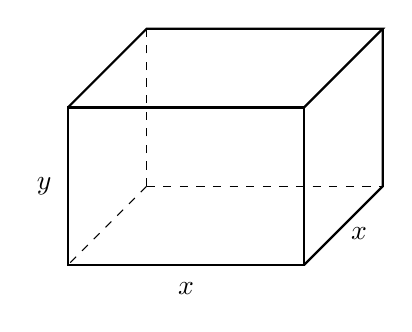
\begin{tikzpicture}
        \draw[dashed] (1,1) -- (1,3);
        \draw[dashed] (1,1) -- (4,1);
        \draw[dashed] (1,1) -- (0,0);

        \draw[thick] (0,0) rectangle (3,2);
        \draw[thick] (3,2) -- (4,3) -- (1,3) -- (0,2);
        \draw[thick] (4,3) -- (4,1) -- (3,0);
        \draw[thick] (0,2) -- (0,0);

        \node at (1.5,-0.3) {\(x\)};
        \node at (-0.3,1) {\(y\)};
        \node at (3.7,0.4) {\(x\)};
    \end{tikzpicture}
\end{center}
\optAs{min}{4xy + x^2}{%
    x^2 y &= 10, \\
    x,y &> 0.
}
Vyjádřeme si jednu proměnnou v závislosti na druhé, například $y = \frac{10}{x^2}$. Následně dosadíme do úlohy a vyšetříme
stacionární body pomocí první derivace.
\[
    \frac{\dif}{\dif y} \left(4x \frac{10}{x^2} + x^2\right)= \frac{-40}{x^2} + 2x \stackrel{!}{=} 0
\]
Zbavme se zlomků:
\begin{align*}
    -40 + 2x^3 &= 0 \\
    x^3 &= 20  \\
    x &= \sqrt[3]{20}
\end{align*}
Tedy jediné možné řešení $x = \sqrt[3]{20} \rightarrow y = \frac{10}{\left(\sqrt[3]{20}\right)^2} =  \sqrt[3]{\frac{5}{2}}$.

% \subsection{Maximalisační úloha}
% V továrně vyrábějí zboží různých druhů. Označme je $X_1, \dots, X_n$. Na jejich výrobu potřebují materiály $Y_1, \dots, Y_m$.
% Na skladě mají k dispozici množství $b_i$ materiálu $Y_i$ a na trhu ho nakupují za cenu $\gamma_i$. Na výrobu jednotkového
% množství zboží $X_j$ potřebují množství $a_{ij}$ materiálu $Y_i$. Jednotkové množství výrobku $X_j$ prodávají za cenu
% $\sigma_j$. Formulujte optimalisační úlohu problému nastavení množství výroby jednotlivých druhů produktů (předpokládejte,
% že hledaná množství nemusí být celočíselná) tak, aby celkový zisk z jejich prodeje byl co největší.
%
\subsection{Optimalisační úloha s nadrovinami}
V $\R^n$ jsou dány množiny bodů $A = \bc{a_1, \dots, a_k}$ a $B = \bc{b_1, \dots, b_t}$. Ať $w \in \R^n$ a $\lambda \in \R$.
Předpokládejme, že $H$ je nadrovina o rovnici $\langle x,w \rangle + \lambda = 0$, $H_1$ je nadrovina o rovnici
$\langle x, w \rangle + \lambda = 1$ a $H_2$ je nadrovina o rovnici $\langle x, w \rangle + \lambda = -1$.
\begin{enumerate}[(a)]
    \item Ukažte, že vzdálenost mezi nadrovinami $H_1$ a $H_2$ je $\frac{2}{||w||}$. Dále ukažte, že $\frac{1}{||w||}$
    je vzdálenost $H$ od $H_1$ a také vzdálenost $H$ od $H_2$.
    \item Iterpretujte optimalisační úlohu
    \optAs{max}{g(w, \lambda) = \frac{2}{||w||}}{%
        &\langle a_i, w \rangle + \lambda \geq 1 &\text{pro všechna } i=1, \dots, k, \\
        &\langle b_i, w \rangle + \lambda \leq -1 &\text{pro všechna } j=1, \dots, l.
    }
    \item Ukažte, že $(\hat w,\hat \lambda)$ je řešením úlohy z předchozího bodu právě tehdy, když je řešením úlohy
    (kvadratického programování) ve tvaru
    \optAs{min}{h(w, \lambda) = \frac{1}{2} ||w||^2}{%
        &\langle a_i, w \rangle + \lambda \geq 1 &\text{ pro všechna } i=1, \dots, k, \\
        &\langle b_i, w \rangle + \lambda \leq -1 &\text{ pro všechna } j=1, \dots, l.
    }
\end{enumerate}

(a) 

\begin{multicols}{2}
  \begin{figure}[H]
    \center
    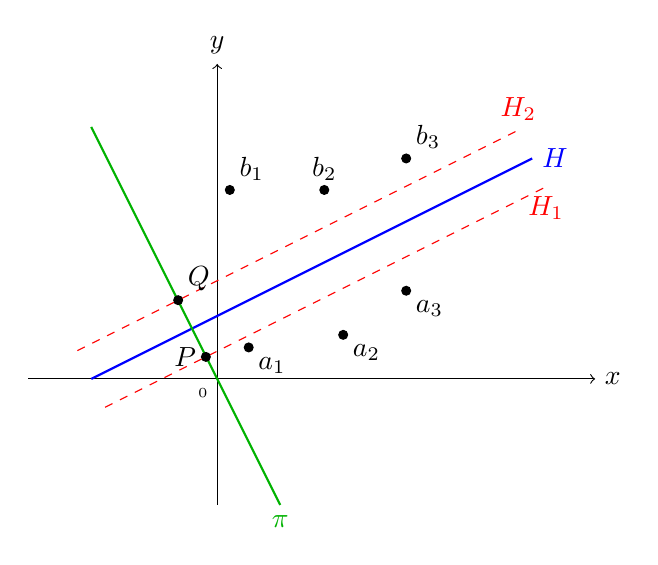
\begin{tikzpicture}[scale=0.8]
        \draw[->] (-3,0) -- (6,0) node[right] {$x$};
        \draw[->] (0,-2) -- (0,5) node[above] {$y$};
      
        \draw[thick,blue] (-2,0) -- (5,3.5) node[right, sloped] {$H$}; % midway
      
        \draw[dashed,red] (-2.22,0.45) -- (4.78,3.95) node[above, sloped] {$H_2$};
        \draw[dashed,red] (-1.78,-0.45) -- (5.22,3.05) node[below, sloped] {$H_1$};
      
        \filldraw[black] (0.5,0.5) circle (2pt) node[below right] {$a_1$};
        \filldraw[black] (2,0.7) circle (2pt) node[below right] {$a_2$};
        \filldraw[black] (3,1.4) circle (2pt) node[below right] {$a_3$};
      
        \filldraw[black] (0.2,3) circle (2pt) node[above right] {$b_1$};
        \filldraw[black] (1.7,3) circle (2pt) node[above] {$b_2$};
        \filldraw[black] (3,3.5) circle (2pt) node[above right] {$b_3$};
    
        \draw[thick,green!70!black] (-2,4) -- (1,-2) node[below, sloped] {$\pi$};
        \filldraw[black] (-0.18,0.35) circle (2pt) node[left] {$P$};
        \filldraw[black] (-0.62,1.25) circle (2pt) node[above right] {$Q$};
    
        \filldraw[black] (0,0) circle(0pt) node[below left] {\tiny 0};
    \end{tikzpicture}
  \end{figure}

\columnbreak

    $\pi : x = t \cdot w, t \in \R$.

    Průsečík $Q$:

    $\underbrace{\langle tw, w\rangle}_{t ||w||^2} + \lambda = 1$ $\rightarrow t = \frac{1-\lambda}{||w||^2}$
    $\Rightarrow Q = \frac{1-\lambda}{||w||^2} w$

    Průsečík $P$:

    $\underbrace{\langle tw, w\rangle}_{t ||w||^2} + \lambda = -1$ $\rightarrow t = \frac{-1-\lambda}{||w||^2}$
    $\Rightarrow P = \frac{-1-\lambda}{||w||^2} w$
\end{multicols}

Pak vzdálenost mezi nadrovinami $H_1$ a $H_2$ je dána rozdílem průsečíků $P$ a $Q$ v normě. Tedy:
\[
    || Q - P || = \left\| \frac{1-\lambda}{||w||^2} w  + \frac{1 + \lambda}{||w||^2} w\right\| = 
    \left\| \frac{2w}{||w||^2} \right\| = \frac{2}{||w||^2} ||w|| = \frac{2}{||w||} \text{.}
\]
To je príma, to jsme přesně chtěli. $\qed$

(b) % TODO: dodělat

(c) V úloze (b) maximalisujeme zlomek, kde se proměnná nachází ve jmenovateli. Tedy snažíme se najít co nejmenší možný
jmenovatel, aby zlomek měl co největší hodnotu. Můžeme úlohu převrátit a minimalisovat samotný jmenovatel. Protože
násobení je lineární a zachovává nám všechny nerovnosti, můžeme různě modifikovat jakou konstantou násobíme námi
minimalisovanou proměnnou. Zároveň si můžeme dovolit umocnit normu, protože i to nám zachová všechny nerovnosti. Zde si 
tedy chytře zvolíme násobení $\frac{1}{2}$, protože při následném hledání stacionárních bodů funkce nám vyskočí z kvadrátu 
dvojka, jenž pěkně pokrátíme. Podmínky nám zůstaly stejné, není co řešit.

% \subsection{Optimalisační úloha se spojnicemi bodů}
% V rovině jsou dány body $P = (0,0)^T$ a $Q = (1,1)^T$.
% \begin{enumerate}[(a)]
%     \item Formulujte optimalisační úlohu problému nalezení nejkratší spojnice bodů $P$ a $Q$. Spojnicí rozumíme křivku
%     danou grafem spojitě diferencovatelné funkce $f : [0,1] \rightarrow \R$.
%     \item Nalezněte řešení úlohy z předchozího bodu.\footnote{Nápověda: Ukažte, že $g(t) = t, t \in [0,1]$, je řešením
%     úlohy. Využijte přitom toho, že pro dvě spojité funkce $f_1$ a $f_2$ na intervalu $[0,1]$ je $\int_0^1 \left(f_1(t),
%     f_2(t) \right)^T \dif T loneq \left(\int_0^1 f_1 (t) \dif t, \int_a^b f_2 (t) \dif t \right)^T$ a platí \\
%     $\left| \left| \int_0^1 (f_1 (t), f_2 (t))^T \dif t \right| \right| \leq \int_0^1 \left| \left| (f_1 (t), f_2 (t))^T \right| \right| \dif t$.
%     K důkazu jednoznačnosti pak lze využít tvrzení, že rovnost v uvedené \uv{trojúhelníkové nerovnosti pro integrály}
%     nastává pávě tehdy, když existuje spojitá funkce $\lambda : [0,1] \rightarrow \R$ taková, že $(f_1 (t), f_2 (t))^T =
%     \lambda (t) \int_0^1 (f_1 (t), f_2 (t))^T \dif t$.
%     }
% \end{enumerate}

% \subsection{Optimalisační úloha s úsečkami}
% V rovině jsou dány body $P = (-1, 0)^T$ a $Q = (1,0)^T$. Ať $L$ je úsečka s krajními body $P$ a $Q$.
% \begin{enumerate} [(a)]
%     \item Formulujte optimalisační plohu problému nalezení spojitě diferencovatelné funkce $y : [-1, 1] \rightarrow \R$,
%     jejíž graf má koncové body $P$ a $Q$, délku $l=3$, leží v horní polorovině a spolu s úsečkou $L$ ohraničuje část
%     roviny o největším obsahu.
%     \item Ať $(x_0, x_1, \dots, x_k)$ je ekvidistantní dělení intervalu $[-1, 1]$ (tj. $x_l = l \delta$, kde
%     $\delta = \frac{2}{k}$). Využitím tohoto dělení k aproximaci integrálu pomocí konečné sumy a derivace pomocí diferencí
%     nalezněte optimalisační úlohu v $\R^{k+1}$, jejíž řešení aproximuje řešení úlohy z předchozího bodu.
% \end{enumerate}

% \subsection{Vztah argmin}
% Ať $\varphi : X \rightarrow Y$ je bijekce, $D_f \subseteq X, D_g \subseteq Y, \varphi(D_f) \subseteq D_g, M \subseteq D_f$
% a $\hat x \in M$. Předpokládejme, že funkce $f : D_f \rightarrow \R$ a $g : D_g \rightarrow \R$ splňují $f = g \circ \varphi$.
% Ukažte, že $\hat x \in \argmin_{x \in M} f(x)$ právě tehdy, když $\varphi (\hat x) \in \argmin_{y \in \varphi (M)} g(y)$.
